\section{Experiments}
\label{sec:experiments}

In this section we provide some experiments to illustrate our theoretical analysis and also the performance of our algorithm. In particular, we evaluate our algorithm on Dudley metric with comparison to the algorithm given by~\cite{sriperumbudur2012empirical}. We show our method is a lot faster and still accurate. We provide a new transport interpretation to this metric of interest. 
\paragraph{Accuracy vs Regularization.} 

\begin{figure}[h!]
\centering
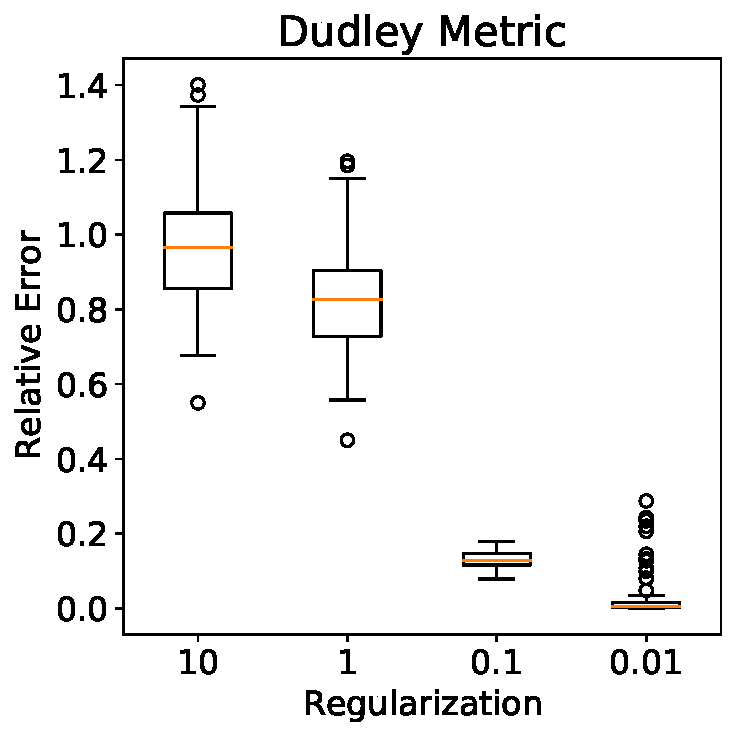
\includegraphics[width=0.8\linewidth]{figures/box_plot_accuracy.pdf}
\caption{Accuracy vs Regularization.\label{fig:result_acc}}
\end{figure}


\paragraph{Time vs Dimension.}

\begin{figure}[h!]
\centering
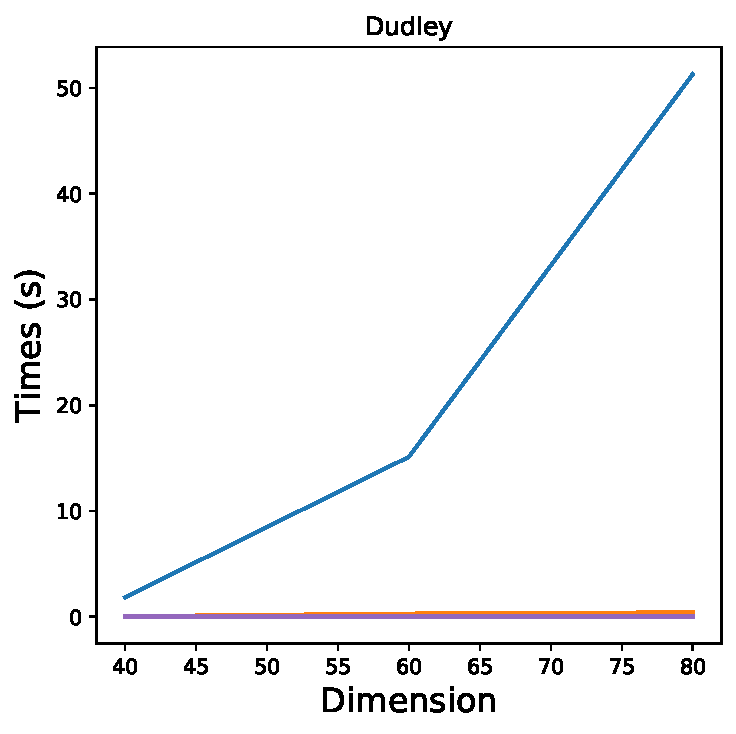
\includegraphics[width=0.3\linewidth]{figures/Time_vs_Dimension.pdf}
\caption{Accuracy vs Regularization.\label{fig:result_acc}}
\end{figure}


The approximation obtained is [PRIMAL formulation]. Explain that this is always bigger than the true value. 



\paragraph{Real Data.}


\section{Conclusion and future work}

In this paper, we defined a new variational problem to deal with multiple costs in Optimal Transport adding the constraints that all the costs must contribute equally to the global transport problem. Primal and dual formulation provides different but coherent interpretations. This helps to understand better the mechanism behind Dudley metric. Following the idea of~\cite{cuturi2013sinkhorn}, we derived an entropic relaxation and an efficient algorithm to approximately compute the solutions to our problem.

We proposed a new way of treating multiple costs in Optimal Transport. There might exist other ways to handle multiple costs and treat them. We leave as further work these other ways. 